\documentclass[10pt,letterpaper,subeqn]{beamer}
\setbeamertemplate{navigation symbols}{}
\usefonttheme{serif}
\usepackage{setspace}
\usepackage{color}
\usepackage[english]{babel}
\selectlanguage{english}
%\usetheme{Dresden}
\usepackage[utf8]{inputenc}
\usepackage{fleqn}
\usecolortheme{orchid}
\usepackage{textcomp}
\usepackage{graphics}
\usepackage{hyperref}
\usepackage{framed}
%\usepackage[pdftex]{graphicx}
\usepackage[update,prepend]{epstopdf}
\usepackage{booktabs}
\setbeamertemplate{caption}[numbered]
\usepackage{upquote}
\usepackage{minted}
\newminted[codepresent]{python}{xleftmargin=0cm}
\AtBeginDocument{%
\def\PYZsq{\textquotesingle}%
}

\usepackage{pgf,tikz}
\usepackage{pgfplots}
\usetikzlibrary{decorations}

\begin{document}
\title{High Powered Data and Development Economics}
\subtitle{Scraping the Web to Generate Unique Datasets}
\author{Damian Clarke}
\date{\today}

\begin{frame}
\titlepage
\end{frame}

\section{Python}
\frame{\frametitle{Why Python?}
\begin{figure}
\vspace{-2.9cm}
\hspace{+5.5cm}

\includegraphics[scale=0.15]{Python2.png}
\end{figure}
\vspace{1cm}
\begin{itemize}
 \item Free
 \item Power over the \emph{whole} operating system
 \begin{itemize}
   \item Imagine if Stata had control over Firefox, image editing, Google Earth, better scientific libraries, \ldots
 \end{itemize}
 \item Quite easy to get up and scraping the web (we'll do it in 20 mins)
 \item If you decide you like it, it can do everything for you
 \begin{itemize}
   \item Kevin Sheppard's course, \href{http://quant-econ.net/}{\textcolor{blue}{John Stachurski and Sargent's course}}
 \end{itemize}
  \item Signalling?
\end{itemize}
}

\frame{\frametitle{What Do You Need?}
\begin{itemize}
 \item Unix or OS X: nothing!
 \item Windows: In many distributions Python is not installed by default
 \begin{itemize}
  \item For complete packages, install Anaconda (\href{http://continuum.io/}{\textcolor{blue}{http://continuum.io/}}) 
 \end{itemize}
 \item It may also be useful to install a stand alone text editor with syntax highlighting (ie gedit)
\end{itemize}

}
%[mathescape,
%               linenos,
%               numbersep=5pt,
%               gobble=2,
%               frame=lines,
%               framesep=2mm]

\frame{\frametitle{How to Run Python}
\begin{itemize}
 \item A number of ways: from the command line, interactively, using ipython 
 \item For the interests of time, we'll just run from the command line 
  \begin{itemize}
   \item However, if you're going to run this frequently, ipython is worth checking out 
  \end{itemize}
 \item If you're interested in following along online (without downloading Python to your local machine), go to \href{http://py-ide-online.appspot.com/}{\textcolor{blue}{http://py-ide-online.appspot.com/}}
\end{itemize}
}

\section{Web Scraping}
\frame{\frametitle{What is Web Scraping?}
Essentially, the process of harvesting data that is directly stored on the web in an irregular or highly disperse format.
\vspace{6mm}
\begin{itemize}
 \item When undertaking econometric analysis, we of course want very regular data, formatted into lines and columns
 \item Generally two steps:
 \begin{itemize}
  \item Looping through nested urls to get to (many) source html pages
  \item Taking html and formatting into a useful structure
 \end{itemize}
  \item There are a number of tools people use for this sort of analysis: Python, R, RapidMiner, even \textsc{Matlab} \ldots
\end{itemize}
}

\frame{\frametitle{Why do we care?}
\begin{itemize}
 \item Often (particularly in developing country settings) data is not stored directly as a csv
 \item In some cases, data does not yet exist in any centralised form
 \item This opens up many entirely different types of data we mightn't have previously thought about
 \item The majority of economics papers are now using `novel' data (ie not survey based)
\end{itemize}

}

\frame{\frametitle{What can we do with it?}
\begin{itemize}
 \item It has come in handy for me many times
\begin{itemize}
 \item Download, unzip and merge 1000+ DHS surveys, up to date at the second that scraping takes place
 \item Download all (30,000+) papers on NBER for text analysis
 \item Download election results: India, Philippines
 \item Repeated calls to World Bank Data Bank
\end{itemize}
 \item And turns up frequently in cool development papers
\begin{itemize}
 \item Looking at effects of natural disasters
 \item Looking at effects of ports
 \item Night lights, geography, bombs, weather, \ldots
\end{itemize}
\end{itemize}
}

\frame{
\begin{figure}
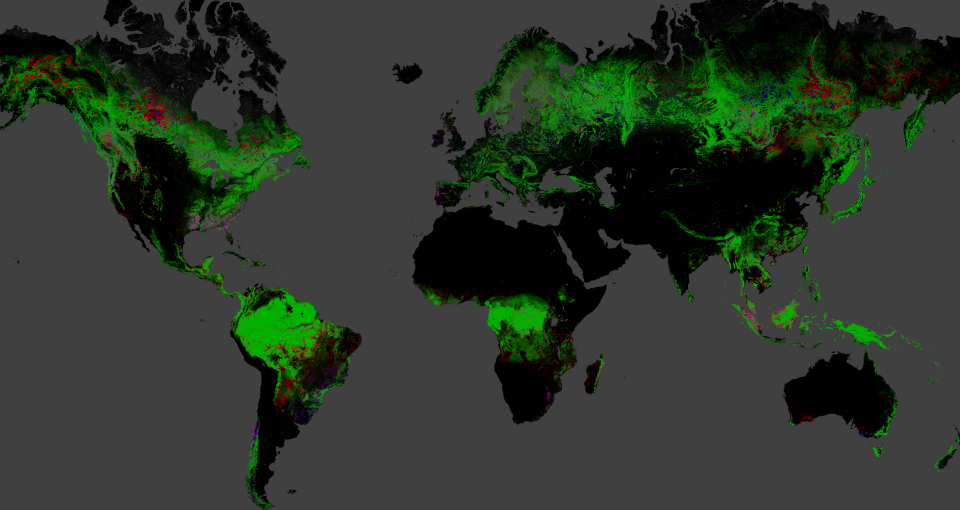
\includegraphics[scale=0.3]{deforestation.png}
\caption{And it can look quite cool\ldots}
\end{figure}
\begin{footnotesize}
Hansen, M.C. et al (2013) High-Resolution Global Maps of 21st-Century Forest Cover Change. \emph{Science} 342 (6160) 850-853. 
\end{footnotesize}
}

\section{Coding}

\frame{\frametitle{Coding}
We will go through a relatively simple (and contrived) example.
\vspace{5mm}
\begin{itemize}
 \item For this process, there are a number of tools we will use:
 \begin{itemize}
 \item Ideally, a web browser that lets us look at source code (pretty much any of them)
 \item Regular Expressions (Python's \texttt{re})
 \item If this is a big job, we should think about error capture (Python's \texttt{try} command)
 \end{itemize}
\end{itemize}
}

\begin{frame}[fragile]
 \frametitle{Basic Code}
 \begin{minted}[mathescape,
               linenos,
               numbersep=5pt,
               frame=lines,
               framesep=3mm,
               fontsize=\scriptsize,
               fontfamily=tt]{python}


#  Scrape_xkcd 0.01             damiancclarke              yyyy-mm-dd:2013-11-21
#---|----1----|----2----|----3----|----4----|----5----|----6----|----7----|----8
#

#*******************************************************************************
# (1) Import required packages, set-up names used in urls
#*******************************************************************************
import urllib2
import re

target = 'http://www.xkcd.com'

#*******************************************************************************
# (2) Scrape target url and print source code
#*******************************************************************************
response = urllib2.urlopen(target)
print response


\end{minted}
\vspace{6mm}
\begin{scriptsize}
If you want to download the source code for the example we'll go through, go to
\href{http://users.ox.ac.uk/~ball3491/Python/}{\textcolor{blue}{http://users.ox.ac.uk/$\sim$ball3491/Python/}}
\end{scriptsize}

\end{frame}

\begin{frame}[fragile]
 \frametitle{Complete Code}
 \begin{minted}[mathescape,
               linenos,
               numbersep=8pt,
               frame=lines,
               framesep=3mm,
               fontsize=\scriptsize,
               fontfamily=tt]{python}
# (1) Import required packages, set-up names used in urls
import urllib2
import re
target = 'http://www.xkcd.com'

# (2) Scrape target url and find the last comic number (num)
response = urllib2.urlopen(target)

for line in response:
    search = re.search('Permanent link to this comic:', line)
    if search!=None:
        lastcomic=re.findall('\d*', line)

for item in lastcomic:
    if len(item)>0:
        num = int(item)

# (3) Loop through all comics, finding each comic's title or capturing errors
for append in range(1, num+1):
    url = target + '/' + str(append)
    response = urllib2.urlopen(url)
    for line in response:
        search = re.search('ctitle',line)
        if search!=None:
            print line[17:-7]
\end{minted}
\end{frame}


\begin{frame}[fragile]
 \frametitle{Or, With Error Capture}
 \begin{minted}[mathescape,
               frame=lines,
               framesep=3mm,
               fontsize=\scriptsize,
               fontfamily=tt]{python}
#*******************************************************************************
# (3) Loop through all comics, finding each comic's title or capturing errors
#*******************************************************************************
for append in range(1, num+1):
    url = target + '/' + str(append)
    try:
        response = urllib2.urlopen(url)
        for line in response:
            search = re.search('ctitle',line)
            if search!=None:
                print line[17:-7]
    except urllib2.HTTPError, e:
        print('%s has http error' % url)
    except urllib2.URLError, e:
        print('%s has url error' % url)


\end{minted}
\end{frame}


\begin{frame}[fragile]
 \frametitle{Exporting Our `Data'}
Python is extremely capable at editing text to create output files:
\vspace{5mm}

 \begin{minted}[mathescape,
               linenos,
               numbersep=8pt,
               frame=lines,
               framesep=3mm,
               fontsize=\scriptsize,
               fontfamily=tt]{python}
#*******************************************************************************
# (3) Loop through all comics, finding each comic's title or capturing errors
#*******************************************************************************
output = open('xkcd_names.txt', 'w')
output.write('Comic, Number, Title \n')

for append in range(1, num+1):
    url = target + '/' + str(append)
    response = urllib2.urlopen(url)
    for line in response:
        search = re.search('ctitle',line)
        if search!=None:
            print line[17:-7]
            output.write('xkcd,' + str(append) + ',' + line[17:-7] + '\n')

output.close()
\end{minted}
\end{frame}

\section{Where to From Here}

\frame{\frametitle{Where to From Here}
\begin{itemize}
 \item You can actually get remarkably far with Python + a web browser + Regular Expressions!
 \item Some times you may want a more structured approach: Beautiful Soup
 \item Python can do much, much, much more
 \item Further applied examples at: \href{https://bitbucket.org/damiancclarke}{\textcolor{blue}{bitbucket.org/damiancclarke}}
 \item Questions/comments?
\end{itemize}
}

\end{document}
